\documentclass{beamer}
%
% Choose how your presentation looks.
%
% For more themes, color themes and font themes, see:
% http://deic.uab.es/~iblanes/beamer_gallery/index_by_theme.html
%
\mode<presentation>
{
%  \usetheme{Berlin}      % or try Darmstadt, Madrid, Warsaw, ...
	\usetheme[
		bullet=circle,                  % Use circles instead of squares for bullets
		titleline=false,                % Show a line below the frame
		alternativetitlepage=true,      % Use the fancy title
		titlepagelogo=logo-sapienza,    % Logo for the first slide
		watermark=watermark-sapienza,   % Watermark used in every slide
		watermarkheight=20px,           % Desired height of the watermark
		watermarkheightmult=6,          % Watermark image is actually x times bigger
	]{Roma}
%  \usecolortheme{beaver} % or try albatross, beaver, crane, ...
%  \usefonttheme{default}  % or try serif, structurebold, ...
%  \setbeamertemplate{navigation symbols}{}
%  \setbeamertemplate{caption}[numbered]
} 

\usepackage[english]{babel}
\usepackage[utf8x]{inputenc}

%other packages...
\usepackage{hyperref}
\usepackage{xspace}
\usepackage{tabularx} % in the preamble
%\usepackage{subfigure}
\usepackage{subfig}
%\usepackage{chngcntr}
%\counterwithin{subfigure}{figure}
% The algorithm packages have to be after hyperref.
\usepackage{algorithm}
\usepackage{algpseudocode}
\usepackage{multirow}
\usepackage{animate}
\usepackage{tasks}

\usepackage{adjustbox}
\usepackage{multimedia}
%\usepackage{movie15}



\usepackage{tikz}
\usetikzlibrary{arrows}
% For every picture that defines or uses external nodes, you'll have to
% apply the 'remember picture' style. To avoid some typing, we'll apply
% the style to all pictures.
\tikzstyle{every picture}+=[remember picture]

% By default all math in TikZ nodes are set in inline mode. Change this to
% displaystyle so that we don't get small fractions.
\everymath{\displaystyle}
\tikzstyle{na} = [baseline=-.5ex]


%%%%%%%%%%%%%%%%%%%%%%%%%% General

\newcommand{\myi}{(\emph{i})\xspace}
\newcommand{\myii}{(\emph{ii})\xspace}
\newcommand{\myiii}{(\emph{iii})\xspace}
\newcommand{\myiv}{(\emph{iv})\xspace}
\newcommand{\myv}{(\emph{v})\xspace}
\newcommand{\myvi}{(\emph{vi})\xspace}
\newcommand{\myvii}{(\emph{vii})\xspace}
\newcommand{\myviii}{(\emph{viii})\xspace}

%% general math
%\newcommand{\A}{\mathcal{A}} 
\newcommand{\B}{\mathcal{B}}
%\newcommand{\C}{\mathcal{C}} 
\newcommand{\D}{\mathcal{D}}
\newcommand{\E}{\mathcal{E}} \newcommand{\F}{\mathcal{F}}
\newcommand{\G}{\mathcal{G}} \renewcommand{\H}{\mathcal{H}}
\newcommand{\I}{\mathcal{I}} \newcommand{\J}{\mathcal{J}}
\newcommand{\K}{\mathcal{K}} \renewcommand{\L}{\mathcal{L}}
\newcommand{\M}{\mathcal{M}} \newcommand{\N}{\mathcal{N}}
\renewcommand{\O}{\mathcal{O}} \renewcommand{\P}{\mathcal{P}}
\newcommand{\Q}{\mathcal{Q}} \newcommand{\R}{\mathcal{R}}
\renewcommand{\S}{\mathcal{S}} \newcommand{\T}{\mathcal{T}}
\newcommand{\U}{\mathcal{U}} \newcommand{\V}{\mathcal{V}}
\newcommand{\W}{\mathcal{W}} \newcommand{\X}{\mathcal{X}}
\newcommand{\Y}{\mathcal{Y}} \newcommand{\Z}{\mathcal{Z}}

\newcommand{\limp}{\mathbin{\rightarrow}}
\newcommand{\ind}{\hspace*{.18in}}

%% LTL
\newcommand{\Next}{\raisebox{-0.27ex}{\LARGE$\circ$}}
\newcommand{\Wnext}{\raisebox{-0.27ex}{\LARGE$\bullet$}}
\newcommand{\Until}{\mathop{\U}}
\newcommand{\Since}{\mathop{\S}}
\newcommand{\Release}{\mathop{\R}}
\newcommand{\Wuntil}{\mathop{\W}}
\newcommand{\true}{\mathit{true}}
\newcommand{\final}{\mathit{Final}}
\newcommand{\false}{\mathit{false}}
\newcommand{\ttrue}{{\mathit{tt}}}
\newcommand{\ffalse}{\mathit{ff}}
\newcommand{\Last}{\mathit{last}}
\newcommand{\Ended}{\mathit{end}}
\newcommand{\length}{\mathit{length}}
\newcommand{\last}{\mathit{n}}
\newcommand{\nnf}{\mathit{nnf}}
\newcommand{\BOX}[1]{ [#1]}
\newcommand{\DIAM}[1]{\langle #1 \rangle}
\newcommand{\transl}{f}


%% Logics
\newcommand{\FOL}{{\sc fol}\xspace}
\newcommand{\LT}{{\sc lt}$_f$\xspace}
\newcommand{\LTi}{{\sc lt}$_i$\xspace}
\newcommand{\LTL}{{\sc ltl}\xspace}
\newcommand{\LTLf}{{\sc ltl}$_f$\xspace}
\newcommand{\LDL}{{\sc ldl}\xspace}
\newcommand{\LDLf}{{\sc ldl}$_f$\xspace}
\newcommand{\RE}{{\sc re}$_f$\xspace}
\newcommand{\REGEX}{{\sc re}\xspace}
\newcommand{\PDL}{{\sc pdl}\xspace}
\newcommand{\FOf}{{\sc fo}$_f$\xspace}
\newcommand{\MSOf}{{\sc mso}$_f$\xspace}
\newcommand{\FO}{{\sc fo}\xspace}
\newcommand{\MSO}{{\sc mso}\xspace}
%\newcommand{\ATA}{{\sc ata}\xspace}
\newcommand{\AFW}{{\sc afw}\xspace}
\newcommand{\NFA}{{\sc nfa}\xspace}
\newcommand{\DFA}{{\sc dfa}\xspace}
\newcommand{\DFAs}{{\sc dfa}s\xspace}
\newcommand{\declare}{{\sc declare}\xspace}
\newcommand{\fol}{\mathit{fol}}
\newcommand{\f}{\mathit{f}}
%\newcommand{\g}{\mathit{g}}
\newcommand{\re}{\mathit{re}}


\newcommand{\tup}[1]{\langle #1 \rangle}

\newcommand{\Stop}{\mathit{stop}}
\newcommand{\rew}{\mathit{rew}}
\newcommand{\Tr}{\mathit{Tr}}

\newcommand{\LOGSPACE}{{\sc logspace}\xspace}
\newcommand{\NLOGSPACE}{{\sc nlogspace}\xspace}
\newcommand{\PTIME}{{\sc ptime}\xspace}
\newcommand{\NP}{{\sc np}\xspace}
\newcommand{\EXPTIME}{{\sc exptime}\xspace}
\newcommand{\PSPACE}{{\sc pspace}\xspace}
\newcommand{\TWOEXPTIME}{{\sc 2exptime}\xspace}


\newcommand{\expand}{\textbf{\textit{E}}}
\newcommand{\ttt}{{\textbf{\textit{T}}}}
\newcommand{\fff}{{\textbf{\textit{\texttt{F}}}}}

\newcommand{\fstate}{s_f}

\newcommand{\atomize}[1]{\texttt{"}\ensuremath{#1}\texttt{"}}


% misc


%RL
\newcommand{\MDP}{\M}
\newcommand{\States}{S}
\newcommand{\Actions}{A}
\newcommand{\TrFun}{T}
\newcommand{\Reward}{R}
\newcommand{\DiscFact}{\gamma}
\newcommand{\Policy}{\rho}
\newcommand{\ExpRet}{G}
\newcommand{\ValFun}{v}
\newcommand{\qFun}{q}

\newcommand{\ValOptFun}{\ValFun^*}
\newcommand{\qOptFun}{\qFun^*}
\newcommand{\OptPolicy}{\Policy^*}

\newcommand{\ValFunEst}{V}
\newcommand{\qFunEst}{Q}
\newcommand{\LRate}{\alpha}

\newcommand{\NMRDP}{\N}
\newcommand{\NMReward}{\bar{\Reward}}
\newcommand{\NMPolicy}{\bar{\Policy}}

%LOGIC

\newcommand{\Prop}{\P}
\newcommand{\PropInt}{\Pi}
\newcommand{\PropFormula}{\phi}
\newcommand{\trace}{\pi}
\newcommand{\Kripke}{\K}
\newcommand{\tm}[1]{\ \text{#1}\ }
\newcommand{\tiff}{\tm{iff}}

\newcommand{\automaton}{\mathcal{A}}
\newcommand{\LLf}{\LTLf/\LDLf}
\newcommand{\DfunSym}{\partial}
\newcommand{\Dfun}[1]{\DfunSym\lparen #1,\PropInt \rparen}
\newcommand{\AND}{\wedge}
\newcommand{\OR}{\vee}
\newcommand{\NOT}{\lnot}
\newcommand{\regexp}{\varrho}
\newcommand{\TrueDelta}[1]{\textit{\textbf{\texttt{T}}}_{#1}}
\newcommand{\FalseDelta}[1]{\textit{\textbf{\texttt{F}}}_{#1}}


\newcommand{\Sapientino}{{\sc sapientino}\xspace}
\newcommand{\Breakout}{{\sc breakout}\xspace}
\newcommand{\Minecraft}{{\sc minecraft}\xspace}

%math

\newcommand{\set}[1]{\{#1\}}
\newcommand{\Naturals}{\mathbb{N}}
\newcommand{\Reals}{\mathbb{R}}
\newcommand{\defeq}{\coloneqq}



%%% Local Variables:
%%% mode: latex
%%% TeX-master: "main"
%%% save-place: t
%%% End:



\usepackage{listings}
% Custom colors
\usepackage{color}
\definecolor{deepblue}{rgb}{0,0,0.5}
\definecolor{deepred}{rgb}{0.6,0,0}
\definecolor{deepgreen}{rgb}{0,0.5,0}
\definecolor{backcolour}{rgb}{0.95,0.95,0.92}
\definecolor{codegray}{rgb}{0.5,0.5,0.5}

\usepackage{accsupp}    
\newcommand{\noncopynumber}[1]{
	\BeginAccSupp{method=escape,ActualText={}}
	#1
	\EndAccSupp{}
}
\lstdefinestyle{Python}{
	language        = Python,
	backgroundcolor=\color{backcolour},
	basicstyle      = \small\ttfamily,
	keywordstyle    = \color{deepblue},
	stringstyle     = \color{deepgreen},
	commentstyle    = \color{codegray}\ttfamily,
	numberstyle=\tiny\color{codegray}\noncopynumber,
	columns=flexible,
	numbers=left,
	stepnumber=1
}

\ifodd\textwidth
\addtolength{\textwidth}{1sp}
\fi


\title[RL for \LLf goals]{Reinforcement Learning for \LLf: Theory and Implementation}
\author{Marco Favorito}
\institute[DIAG at Sapienza, Rome]{M.Sc. in \\Engineering in Computer Science \\at Sapienza, University of Rome}
\date{A.Y. 2017/2018}
%Advisor: prof. Giuseppe De Giacomo



\begin{document}

\begin{frame}[t, plain]
  \titlepage
\end{frame}

% Uncomment these lines for an automatically generated outline.
%\begin{frame}{Outline}
%  \tableofcontents
%\end{frame}

%\section{Introduction}

\begin{frame}{Introduction}
\begin{itemize}
	\item Classic Reinforcement Learning:
		\begin{itemize}
			\item 	An \emph{agent} interacts with an \emph{environment} by taking \emph{actions} so to maximize \emph{rewards};
			\item 	No knowledge about the transition model, but assume Markov property (history does not matter);
			\item 	Based on Markov Decision Process (MDP)
		\end{itemize}
		
	\vskip 0.5cm
	\item RL for Non-Markovian Decision Process (NMRDP):
		\begin{itemize}
			\item 	Rewards depend from history, not just the last transition;
			\item 	Specify proper behaviours by using temporal logic formulas;
			\item 	Reduce the problem to MDP (with extended state space)
		\end{itemize}
	
	\vskip 0.5cm
	\item In (Brafman et al. 2018) specify reward using:
			\begin{itemize}
				\item 	Linear-time Temporal Logic on Finite Traces \LTLf 
				\item 	Linear-time Dynamic Logic on Finite Traces  \LDLf
			\end{itemize}	

\end{itemize}
\end{frame}

%\begin{block}{Examples}
%Some examples of commonly used commands and features are included, to help you get started.
%\end{block}



%\section{Some \LaTeX{} Examples}

%\subsection{Tables and Figures}

\begin{frame}{Example of NMRDP: \Breakout}
	\begin{itemize}
		\item Non-Markovian reward: remove columns from left to right
		\item The solution space is restricted
		\item Policy must depend from a sequence of states: $\Policy: S^* \to A$
	\end{itemize}

	\begin{figure}
		\centering
		
\includegraphics[width=0.5\textwidth]{images/breakout.jpg}
	\end{figure}
\end{frame}



\begin{frame}{Goals of the thesis}

\begin{itemize}
\item Theoretical foundations for RL over NMRDP with \LLf rewards by leveraging (Brafman et al. 2018)

\vskip 0.5cm

\item Formalization and solution of a new problem: RL for \LLf goals 
\begin{itemize}
	\item two-fold representation of the world
	\begin{itemize}
		\item Low-level, used by the learning agent 
		\item High-level, used to specify the goal formulas 
	\end{itemize}


\end{itemize}

\vskip 0.5cm

\item Deal with sparse rewards and design a way to improve exploration

\vskip 0.5cm

\item Implementation of the topics described above

\end{itemize}

\end{frame}

%\subsection{Mathematics}

\begin{frame}{\LTLf and \LDLf (De Giacomo and Vardi, 2013)}
	\begin{itemize}
		\item Linear Temporal Logic on finite traces: \LTLf
			\begin{itemize}
				\item Exactly the same syntax of \LTL
				\item Interpreted over finite traces
	
			\begin{tasks}[counter-format = -](2)
				\task Next: $\Next happy$
				\task Until: $reply \lUntil acknowledge$
				\task Eventually: $\Diamond rich$
				\task Always: $\Box safe$
			\end{tasks}
%			\[\begin{array}{rcl}
%			\varphi &::=& \Atom \mid \lnot \varphi \mid \varphi_1\land \varphi_2 \mid \Next\varphi \mid \varphi_1 \lUntil \varphi_2
%			\end{array}
%			\]
			
			\end{itemize}

	
		\item Linear Dynamic Logic on finite traces: \LTLf
			\begin{itemize}
				\item Merging of \LTLf and Regular Expressions
	
				\begin{tasks}[counter-format = -](2)
					\task $\BOX{true^*}(safe)$
					\task $\DIAM{A^*;B}End$
				\end{tasks}
%			\[\begin{array}{lcl}
%			\varphi &::=& \ttrue  \mid \lnot \varphi \mid \varphi_1 \land \varphi_2 \mid \DIAM{\varrho}\varphi \\
%			\varrho &::=& \phi \mid \varphi? \mid  \varrho_1 + \varrho_2 \mid \varrho_1; \varrho_2 \mid \varrho^*
%			\end{array}
%			\]
			\end{itemize}
		
		\item Reasoning in \LLf:
			\begin{itemize}
				\item transform formulas $\varphi$ into NFAs or DFAs $\automaton_\varphi$
				\item For every trace $\trace$ and \LLf formula $\varphi$: \[\trace \models \varphi \iff \trace \in \L(\automaton_\varphi)\]
			\end{itemize}
	\end{itemize}
\end{frame}


\begin{frame}{From \LLf formulas to automata: examples}
E.g. For $\trace = \tup{\set{}, \set{A}, \set{A, B}}$, 
\begin{table}
	\centering
\begin{tabular}{c c c} 
	$\trace \not\models \Box A$ & $\trace \models \Diamond A$ & $\trace \not\models \DIAM{(A;B)^*}End$\\
    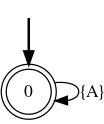
\includegraphics[width=.20\textwidth]{images/ltlf-alwaysA-dfa-no-borders} & 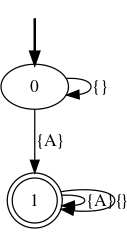
\includegraphics[width=.20\textwidth]{images/ltlf-eventuallyA-dfa-no-borders} & 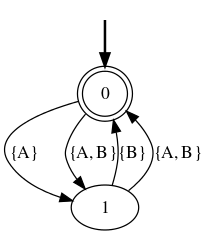
\includegraphics[width=.35\textwidth]{images/alternating-sequence-dfa-no-borders} \\
   	$\Box A$ & $\Diamond A$ & $\DIAM{(A;B)^*}End$ \\
   	\emph{Always A} & \emph{Eventually A} & \emph{Alternating $A$ and $B$} \\ 
\end{tabular}\\
\end{table}


% \begin{figure}
% 	\centering
% 	\subfloat[$\Box A$: “always A . Till the end of the trace, A holds”
% 	\label{fig:a}]{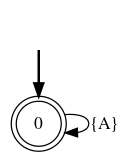
\includegraphics[width=0.25\textwidth]{images/ltlf-alwaysA-dfa}}\qquad
% 	\subfloat[$\Diamond A$: “Eventually A. Sooner or later, A holds”
% 	\label{fig:b}]{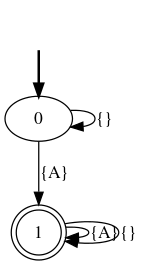
\includegraphics[width=0.25\textwidth]{images/ltlf-eventuallyA-dfa}}\qquad
% 	\subfloat[$\DIAM{(A;B)^*}End$: “Eventually A. Sooner or later, A holds”]{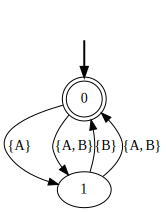
\includegraphics[width=0.25\textwidth]{images/alternating-sequence-dfa}}
%% 	\caption{A figure}
%% 	\label{fig:1}
% \end{figure}
%	
\end{frame}

\begin{frame}[fragile]{FLLOAT: From \LLf tO AutomaTa}

\begin{itemize}
	\item Python package supporting:
	\begin{itemize}
		\item \LLf formulas: parsing, syntax and semantics
		\item Translation to automata (\NFA, \DFA, on-the-fly \DFA)
	\end{itemize}

		\item $\Box A$:
\begin{lstlisting}[language=Python, style=Python, numbers=none]
from flloat.parser.ltlf import LTLfParser
parser = LTLfParser()
always_A = parser("G(A)")
dfa = always_A.to_automaton(determinize=True)
dfa.to_dot("always_A.svg")
\end{lstlisting}

%					\begin{figure}
%						\includegraphics[width=0.75\textwidth]{images/flloat-code-always-example}
%					\end{figure}
			\item $\DIAM{(A;B)^*}End$:
\begin{lstlisting}[language=Python, style=Python, numbers=none]
from flloat.parser.ldlf import LDLfParser
parser = LDLfParser()
alternating_AB = parser("<(A;B)*>end")
dfa = alternating_AB.to_automaton(determinize=True)
dfa.to_dot("alternating_AB.svg")
\end{lstlisting}
	\end{itemize}

\end{frame}

\begin{frame}{RL for NMRDP with \LLf rewards}
	\begin{itemize}
		\item Given an NMRDP $\NMRDP$ with:
		\begin{itemize}
			\item rewards specified by \LLf formulas 
			\item over a set of propositional symbols $\Prop$
			\item agent’s state space: $S \subseteq 2^\Prop$
		\end{itemize}
		\item 	We can transform it into an equivalent MDP $\MDP$ (Brafman et al. 2018)
		\begin{itemize}
			\item the state space of $\MDP$ is extended:\\
					\[S' = S \times Q_1 \times \dots \times Q_m\]
				where $Q_i$ is the set of states of $\automaton_{\varphi_i}$
				
			\item 	reward is given iff $q_i$ is an accepting state of $\automaton_{\varphi_i}$
		\end{itemize}

		\item An optimal policy for $\MDP$ is optimal for $\NMRDP$
		\item We reduced RL for $\MDP$ to RL for $\NMRDP$

		
	\end{itemize}
	
	
\end{frame}


\begin{frame}{RL for \LLf goals: a new problem}
	
		\textbf{Two-fold representation} of the world $\W$:
		\begin{itemize}
			\item An agent learning an MDP with \textbf{\emph{low-level} features} $S$, trying to optimize reward $R$
			\item \LLf goals $\set{(\varphi_i, r_i)_{i=1}^m}$ over a set of \textbf{\emph{high-level} features} $\F$, yielding a set of fluents configurations $\L = 2^\F$
		\end{itemize}
		
		\textbf{Solution}: a non-Markovian policy $\Policy: S^*\to A$ that is optimal wrt rewards $r_i$ and $R$.
		
		\begin{figure}
			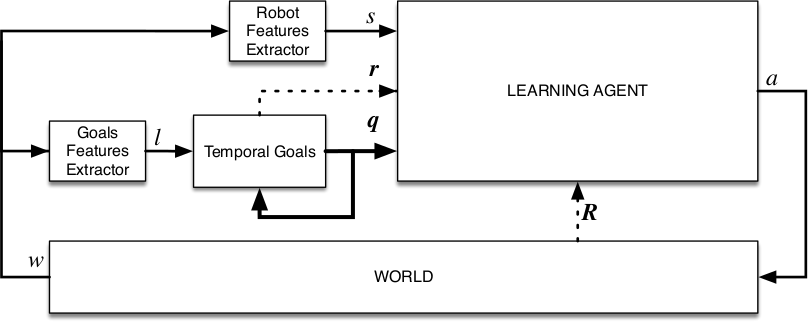
\includegraphics[width=0.75\textwidth]{images/rl-two-representations-no-borders}
		\end{figure}
		
%		Notice: we have to deal with a joint transition model:
%		\[Tr' = S \times \L \times A \to Prob(S, \L) \]
			
\end{frame}

\begin{frame}
	Our approach:
	\begin{itemize}
		\item Transform each $\varphi_i$ into \DFA $\automaton_{\varphi_i}$
		\item Do RL over an MDP $\MDP'$ with a transformed state space:
		\[S'= 
		\tikz[baseline]{
			\node[fill=yellow!20,anchor=base] (ts)
			{$S$};
		}
		\times 
		\tikz[baseline]{
			\node[fill=blue!20,anchor=base] (tq)
			{$Q_1 \times \dots \times Q_m$};
		}
		\]
	\end{itemize}
	
%	\begin{tikzpicture}
%	\end{tikzpicture}
	
	\begin{tikzpicture}
	\node[anchor=south west,inner sep=0] at (0,0) {		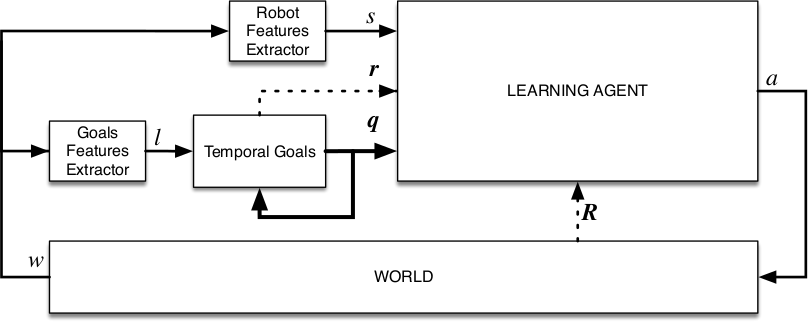
\includegraphics[width=0.9\textwidth]{images/rl-two-representations-no-borders}};
%	\draw[red,ultra thick,rounded corners] (7.5,5.3) rectangle (9.4,6.2);
%	\node [draw=red, anchor=base] (sl) at (1.95,2.25) {};
	\node [anchor=base] (sl) at (1.95,2.3) {};
	\node [anchor=base] (ss) at (4.65, 3.8) {};
	\node [anchor=base] (sq) at (4.65, 2.5) {};
	\end{tikzpicture}
	
%	\begin{figure}
%		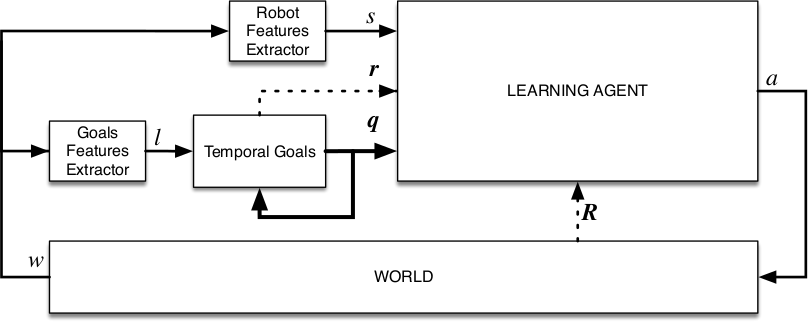
\includegraphics[width=0.9\textwidth]{images/rl-two-representations-no-borders}
%	\end{figure}
		Notice: \textbf{the agent ignores the fluents} \tikz[baseline]{\node[fill=red!20,anchor=base] (tl) {$\L$}}!\\
		
		
		The actual RL relies on standard RL algorithms (e.g. Sarsa($\lambda$))
	
	% Now it's time to draw some edges between the global nodes. Note that we
	% have to apply the 'overlay' style.
	\begin{tikzpicture}[overlay]
	\path[->]<1-> (ts) edge [bend left] (ss);
	\path[->]<1-> (tq) edge [bend left] (sq);
	\path[->]<1-> (tl) edge [bend right] (sl);
	\end{tikzpicture}
	
\end{frame}

\begin{frame}{Automata-based Reward Shaping}
	\begin{itemize}
		\item \emph{Reward sparsity} is the main issue: \textbf{Hard to learn complex behaviors without heuristics}
	\end{itemize}

	

	
	\textbf{Idea}: Give additional reward if, after a transition on $\automaton_\varphi$, we are closer to an accepting state (anticipate rewards)
	
	Based on \emph{Potential-Based Reward Shaping} (Ng et al., 1999):
	\[F(s,a,s') = \DiscFact\Phi(s') - \Phi(s)\]
	
	Two modes:
	\begin{itemize}
		\item \emph{Off-line}: $\Phi(q)$ inversely proportional to the distance from any accepting state of $\automaton_\varphi$ 
		\item \emph{On-line}: $\automaton_\varphi$ and $\Phi$ are built from scratch and updated while learning and discovering new states/transitions. Using \emph{Dynamic PBRS} (Devlin, 2012)
	\end{itemize}
	
\end{frame}

\begin{frame}[fragile]{RLTG (Reinforcement Learning for Temporal Goals)}
	Reinforcement Learning Python framework that implements our approach
	\begin{itemize}
		\item Depends on \texttt{flloat} for the construction of $\automaton_{\varphi_i}$
		\item Works also for classic RL
		\item Highly customizable, uses OpenAI Gym interface
	\end{itemize}
	Example (in pseudocode):
\begin{lstlisting}[language=Python, style=Python, numbers=none, escapechar = £]
env = GymEnvironment()           # a Gym environment 
agent = TGAgent(                 # the "temporal goal" agent
    FeatureExtractor(...),       # generates the agent's space
    Brain(...), #abstraction of RL algorithms (e.g. Sarsa)
    [TemporalGoal(£$\varphi, r$£), ...] # list of temp. goal managers
)
trainer = TGTrainer(env, agent, stop_conditions=..., ...)
trainer.main(...)                # starts the learning process

\end{lstlisting}
\end{frame}


\begin{frame}{Experiments: \Breakout}
\Breakout: remove columns/rows in a given order
	\begin{itemize}
		\item \textbf{low-level features}: paddle position, ball speed/position;
		\item \textbf{high-level features}: bricks status (broken/not broken)
		\item \textbf{\LLf goal} ($l_i$ means: the $i_{th}$ line has been removed.):
		\[\DIAM{(\lnot l_0 \lAND \lnot l_1 \lAND \lnot l_2)^*;(l_0 \lAND \lnot l_1 \lAND \lnot l_2);(l_0 \lAND \lnot l_1 \lAND \lnot l_2)^*;\dots;(l_0 \lAND l_1 \lAND l_2)}tt\]
	\end{itemize}
	%\animategraphics[width=\textwidth]{12}{gifs/frame-}{0}{18}
	\begin{table}
		\centering
		\begin{tabular}{c c}
		 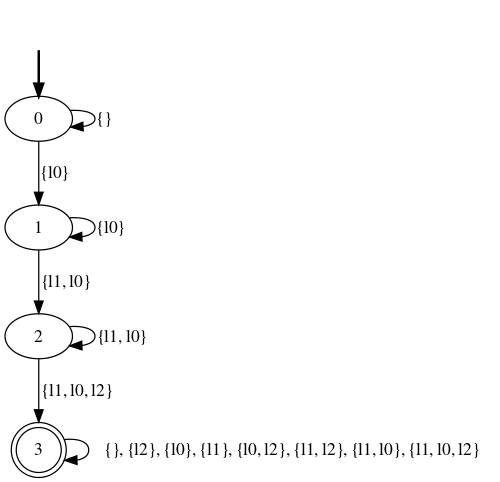
\includegraphics[width=.35\textwidth]{images/breakout.png} &
			\movie[height = 3.5cm, width = 4cm, showcontrols,	poster]{}{breakout-left-right.avi}
		\end{tabular}
	\end{table}

	
\end{frame}

\begin{frame}{Experiments: \Sapientino}
	\Sapientino: make a \emph{bip} in each color, in a given order
	\begin{itemize}
		\item \textbf{low-level features}: robot position $(x, y)$;
		\item \textbf{high-level features}: color of current cell, bip-last-action
		\item \textbf{\LLf goal}:
		\[\DIAM{(¬bip)^* ;red \wedge bip; (¬bip)^*;green \wedge bip; \dots}tt\]
	\end{itemize}
	
	%\animategraphics[width=\textwidth]{12}{gifs/frame-}{0}{18}
	\begin{table}
		\centering
		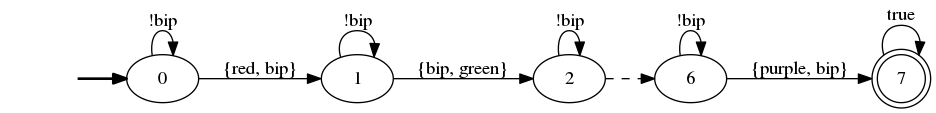
\includegraphics[width=0.6\textwidth]{images/sapientino_ldlf_horizontal}
		\begin{tabular}{c}
			\movie[height = 3.7cm, width = 4cm, showcontrols,	poster]{}{sapientino.avi}
		\end{tabular}
	\end{table}

\end{frame}

\begin{frame}{Experiments: \Minecraft}
	\Minecraft: complete tasks by getting resources/using tools
	\begin{itemize}
		\item \textbf{low-level features}: robot position $(x, y)$;
		\item \textbf{high-level features}: $get\_wood$, $use\_workbench$ etc.
		\item \textbf{\LLf goal}: three composite tasks like (approximately):
		\[
		\DIAM{\true^*}\DIAM{get\_iron ; get\_iron \lAND get\_wood; \dots \lAND use\_factory}tt
		\]
	\end{itemize}
	
	%\animategraphics[width=\textwidth]{12}{gifs/frame-}{0}{18}
	\begin{table}
		\centering
		\begin{tabular}{c c}
			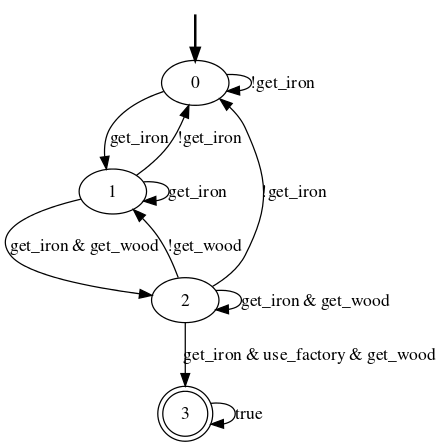
\includegraphics[width=0.3\textwidth]{images/minecraft_goals_no_borders} &
			\movie[height = 3.7cm, width = 4cm, showcontrols,	poster]{}{minecraft.avi}
		\end{tabular}
	\end{table}
	
\end{frame}



\begin{frame}{Discussion}

	Why a two-fold representation for temporal goals?
	\begin{itemize}
		\item \emph{Separation of concerns}: It allows to a better design of the RL system by improving modularity and flexibility;
		\item \emph{Reduced state space}: It makes easier the learning by exploring a smaller state space and focusing only on relevant low-level features;
		\item \emph{Simpler agent}: Move part of the complexity outside the agent.
	\end{itemize}
	Other observations:
	\begin{itemize}
		\item \emph{Expressive Power}: \LDLf expressive as Monadic Second-Order logic (e.g. we can specify procedural constraints);
		\item No need of new algorithms, one can rely on off-the-shelf RL algorithms (Sarsa($\lambda$), Q-Learning, ...);
		\item The correlation between the two representations does not need to be formalized.
	\end{itemize}

\end{frame}

\begin{frame}{Conclusions}
	Thesis results:
	\begin{itemize}
		\item Extended (Brafman et al. 2018) to the context of RL;
		\item Formalization of \emph{RL for \LLf goals}, devising of a solution and analysis of the advantages;
		\item Provided an implementation and given experimental evidence of the goodness of our approach.
	\end{itemize}
	Future works:
	\begin{itemize}
		\item Minimal low-level representation to tackle \LLf goals;
		\item Optimize FLLOAT, enrich RLTG;
		\item Try the approach in several real world applications;
		\item Design of ad-hoc algorithms (e.g. "automata-aware" exploration);
		\item Extend the approach to the framework of Multi-Agent Systems.
	\end{itemize}
	Publication: \href{https://arxiv.org/abs/1807.06333}{https://arxiv.org/abs/1807.06333}. Status: submitted
	
\end{frame}

\end{document}
